\documentclass[12pt]{mwart}

\usepackage{polski}
\usepackage[utf8]{inputenc}
\usepackage{mathtools,amsthm,amssymb,icomma,upgreek,xfrac,graphics,scrextend,float,tabularx,hyperref,multicol,array,caption,enumitem}
\usepackage[table,xcdraw]{xcolor}

\mathtoolsset{mathic}
\raggedbottom
\graphicspath{ {./images/} }
\renewcommand{\refname}{Źródła}
\captionsetup{justification=raggedright,singlelinecheck=true}


\begin{document}
	
	\begin{center}
		{\Large\textbf{Symulacje komputerowe}}
	\end{center}
	\begin{center}
		Raport 2
	\end{center}
	
	\noindent Temat: \ \textbf{Proces Ryzyka i ruch Browna}\\
	Imię i Nazwisko prowadzącego kurs: \ \textbf{Dr Michał Balcerek}	\newline\newline
	
	
	\noindent\begin{tabularx}{\textwidth}{|X |X|}
		\hline
		\begin{center}
			Imię i Nazwisko,\\ nr indeksu
		\end{center} &  \begin{center}
			Kacper Brudnik, 262286\\
			Szymon Malec, 262276
		\end{center}\\\hline
		Wydział: & Wydział matematyki, W13 \\\hline
		Dzień i godzina zajęć: & Wtorek,\vphantom{ $11^{1^{5}}$} $11^{15}$\\\hline
		Kod grupy ćwiczeniowej: & T00-70d \\\hline
		Data oddania raportu: & 26.06.2022 \\\hline
		\textbf{Ocena końcowa} &\\\hline
	\end{tabularx}\newline\newline
	
	\noindent\textbf{Adnotacje i uwagi:}
	
	\newpage
	
	
	\section{Wstęp}
	\noindent 
	
	
	
	\section{Zadanie 1}

	\subsection{Jednorodny proces Poissona}
	
	\noindent Jednorodnym procesem Poissona z intensywnością $\lambda > 0$ nazywamy proces liczący $\{N_t\}_{t \geq 0}$, który spełnia:
	\begin{itemize}
		\item $N_0 = 0$,
		\item $N_t$ ma niezależne przyrosty,
		\item $N_t$ ma stacjonarne przyrosty,
		\item $N_t \sim \mathcal{P}oiss(\lambda t)$.
	\end{itemize}
	Proces ten służy do zliczania wystąpień pewnych zdarzeń losowych, których częstość występowania (intensywność) jest cały czas taka sama.\\
	
	\noindent Do symulacji procesu Poissona przydaje się jedna z jego własności, którą jest to, że odstępy czasowe pomiędzy skokami mają rozkład $\mathcal{E}xp(\lambda)$.
	Oznacza to, że jeśli chcemy wygenerować jedną trajektorię na przedziale $[0, T]$, to wystarczy generować kolejne $X_i \sim \mathcal{E}xp(\lambda)$, aż ich suma przekroczy $T$.\\
	
	\noindent \textbf{Algorytm}
	\begin{enumerate}
		\item Definiuj $I = 0$, $t=0$.
		\item Generuj $X \sim \mathcal{E}xp(\lambda)$.
		\item $t = t + X$. Jeśli $t > T$, przerwij i zwróć $\{S_i\}$. W przeciwnym razie $I = I + 1$, $S_I = t$.
		\item Wróć do kroku 2.
	\end{enumerate}
	Otrzymane z powyższego algorytmu $\{S_i\}$ to czasy oczekiwania na i-ty skok od startu trajektorii.
	
	
	
	\subsection{Klasyczny proces Ryzyka}
	
	\noindent Klasycznym procesem Ryzyka nazywamy proces stochastyczny opisujący kapitał firmy ubezpieczeniowej postaci
	$$ R_t = u + ct - \sum_{i=1}^{N_t} X_i, $$
	gdzie
	\begin{itemize}[label=\textbf{.}]
		\item $u > 0$ -- kapitał początkowy,
		\item $ct$ -- stałe przychody ($c > 0$),
		\item $N_t$ -- jednorodny proces Poissona z intensywnością $\lambda > 0$,
		\item $X_i$ -- ciąg niezależnych zmiennych losowych o tym samym rozkładzie opisujący straty, $\mathrm{E}X_i = \mu$, $X_i > 0$.
	\end{itemize}
	Proces ten odgrywa ważną rolę w branży ubezpieczeniowej, ponieważ symulacja tego procesu pozwala oszacować prawdopodobieństwo bankructwa firmy oraz jej średni zysk. Dzięki temu jesteśmy w stanie określić jaka powinna być cena ubezpieczenia, by takie prawdopodobieństwo nie było zbyt wysokie, a zysk zadowalający.\\
	
	\noindent Parametrem odpowiadającym za przychody jest stała $c$. Do odpowiedniego doboru tego parametru wykorzystuje się wzór
	$$ c = (1 + \theta)\mu\lambda, $$
	gdzie $\theta > 0$ jest parametrem odpowiadającym za wysokość premii.\\
	
	\noindent \textbf{Algorytm}
	\begin{enumerate}
		\item Generuj $N_t$ na przedziale $[0, T]$.
		\item Generuj $X_1, \dots, X_{N_t}$.
		\item Zwróć $R_t = u + ct - \sum\limits_{i=1}^{N_t} X_i$.
	\end{enumerate}
	
	
	
	\subsection{Dopasowanie modelu do danych}
	
	\noindent Zastosujemy teraz proces Ryzyka w praktyce. Postaramy się jak najlepiej dopasować model klasycznego procesu Ryzyka do danych, które zostały nam udostępnione przez prowadzącego zajęcia laboratoryjne. Dane te opisują 50 trajektorii pewnego klasycznego procesu Ryzyka. Naszym celem jest wyznaczenie parametrów tego procesu na podstawie danych, by móc następnie przeprowadzać jego symulacje.\vspace{2mm}\\
	Badany proces został wysymulowany na odcinku $[0, 100]$ z krokiem czasowym $h = 0,01$. Kapitał początkowy wynosi $u = 50$.
	
	\subsubsection{Parametr {\boldmath $c$}}
	\noindent Możemy wyznaczyć go w bardzo prosty sposób. Wiedząc, że jest to współczynnik nachylenia funkcji liniowej $ct$, wystarczy, że policzymy o ile funkcja ta wzrasta w jednym kroku czasowym (obliczymy różnicę dwóch sąsiadujących danych) i wartość tę podzielimy przez długość kroku. Ważne, by upewnić się, czy w danym kroku nie nastąpił spadek. Dla pewności możemy policzyć $c$ dla kilku kroków i sprawdzić, czy otrzymane wartości są identyczne. Wartość, którą otrzymaliśmy z naszych danych to $c = 56,25$.
	
	\subsubsection{Parametr {\boldmath $\lambda$}}
	\noindent W przypadku tego parametru nie jesteśmy w stanie wyznaczyć jego dokładnej wartości, zatem skorzystamy z estymatora. Wykorzystamy fakt, że jeśli proces Poissona ma intensywność $\lambda$, to odstępy czasowe między kolejnymi skokami mają rozkład $\mathcal{E}xp(\lambda)$. Wydzielamy więc wszystkie czasy oczekiwania ze wszystkich trajektorii do jednego zbioru danych. Robimy to sumując wszystkie kroki czasowe następujące po każdym spadku aż do następnego spadku, przy czym dodajemy także ostatni krok spadkowy. Należy zaznaczyć w tym miejscu, że pozwalamy sobie tutaj na pewne uproszczenie, ponieważ przyjmujemy, że spadek miał miejsce dokładnie pod koniec kroku spadkowego, podczas gdy w rzeczywistości miał on miejsce w jego trakcie.\vspace{2mm}\\
	By wyestymować parametr $\lambda$, skorzystamy z faktu, że dla $\tau \sim \mathcal{E}xp(\lambda)$ wartość oczekiwana jest równa
	$$ \mathrm{E}\tau = \frac{1}{\lambda}. $$
	Najlepszym estymatorem wartości oczekiwanej jest średnia z próby. Oznaczmy przez $\tau_1, \dots, \tau_n$ odstępy czasowe pozyskane z naszych danych. Estymatorem $\lambda$ będzie więc
	$$ \widehat{\lambda} = \frac{1}{\sum\limits_{i=1}^n \tau_i}. $$
	Po obliczeniu otrzymaliśmy $\widehat{\lambda} \approx 1,48$. Poniżej możemy zobaczyć, że krzywa gęstości teoretycznej rozkładu $\mathcal{E}xp\left(\widehat{\lambda}\right)$ wyraźnie pokrywa się z histogramem z naszych danych.
	
	\begin{figure}[H]
		\centering
		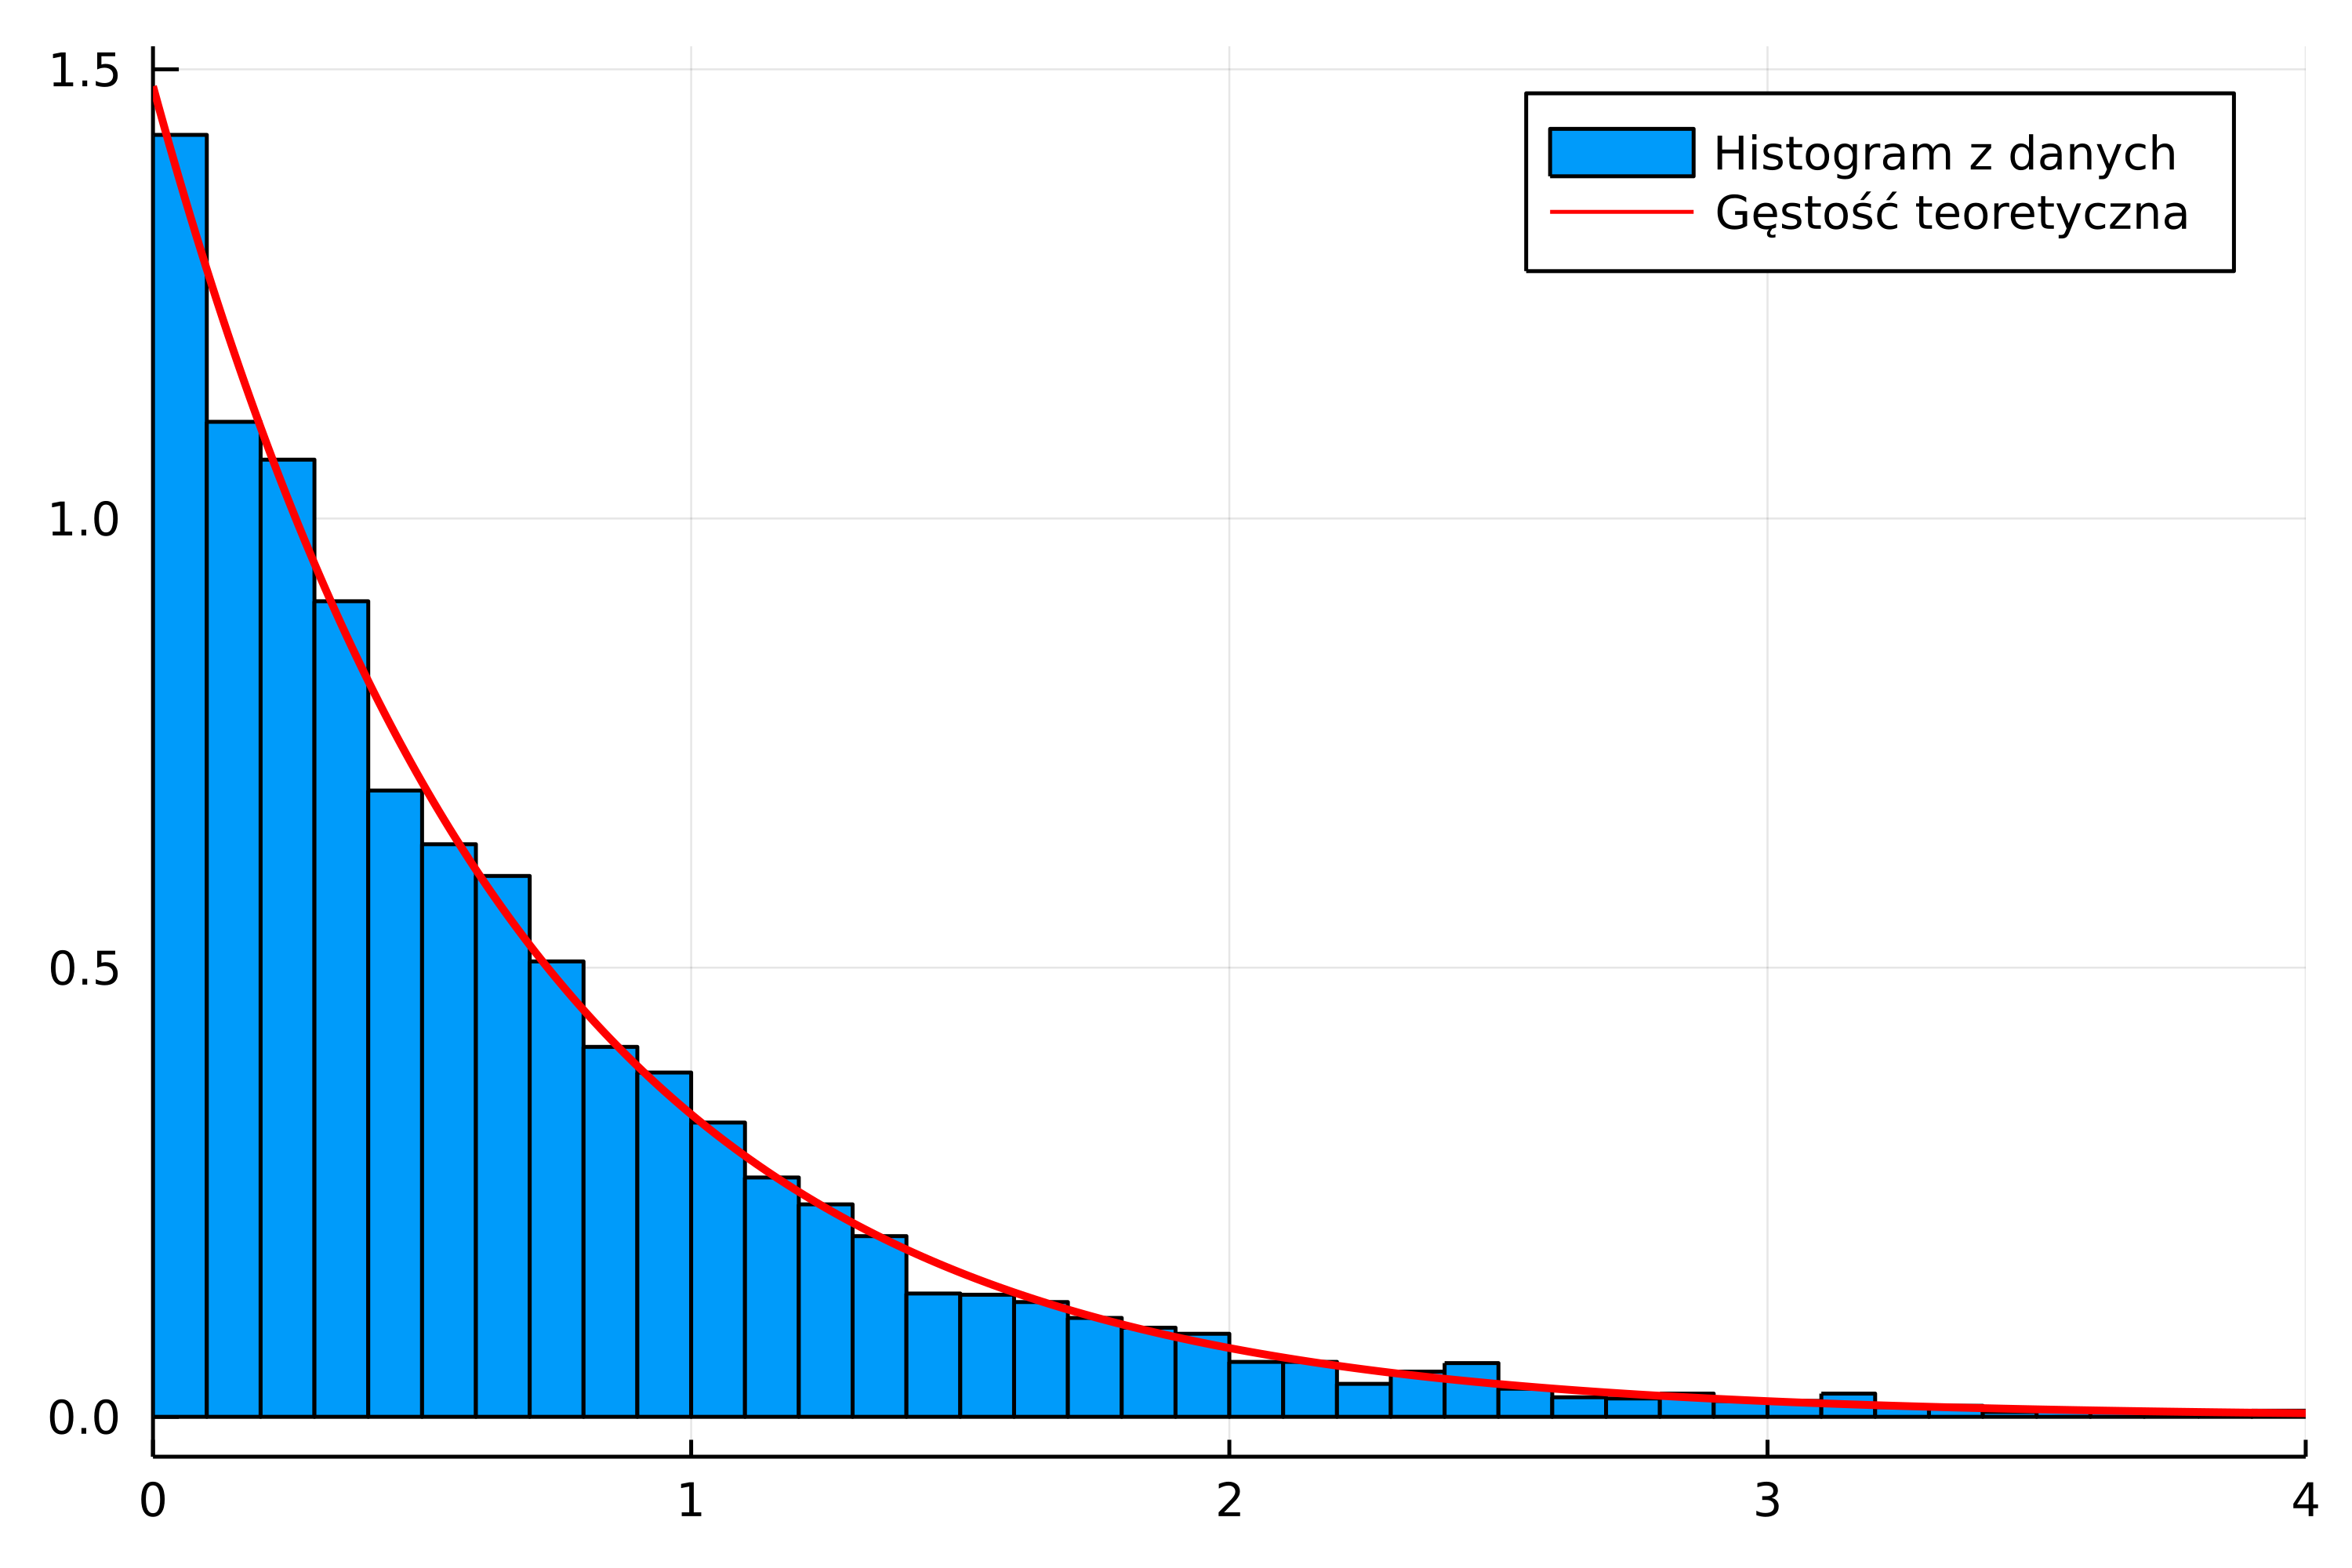
\includegraphics[scale=0.1]{fig/lambda.png}
		\caption{Porównanie histogramu z odstępów czasowych pomiędzy skokami z gęstością teoretyczną rozkładu $\mathcal{E}xp\left(\widehat{\lambda}\right)$.}
	\end{figure}
	
	\subsubsection{Straty {\boldmath $X_i$}}
	
	\subsubsection{Parametr {\boldmath $\theta$}}
	
	
	
	\subsection{Prawdopodobieństwo ruiny}
	
	
	
	
	\section{Zadanie 2}
	
	
	
	\section{Podsumowanie}
	
	
	
	\newpage
	\begin{thebibliography}{1}
		\bibitem{dane}
		\url{}
	\end{thebibliography}


\end{document}